%-----------------------------------------------------------------------------%
\chapter{LANDASAN TEORI}
Pada bab ini akan dijelaskan teori pendukung serta metode yang digunakan untuk mengekstraksi modul-modul yang terdapat pada aplikasi monolitik. Penjelasan teori dimulai dengan pengertian dari arsitektur Microservice, prinsip dan pemodela microservice, membangun arsitktur microservice dari arsitektur monolitik, metode pengembangan aplikasi berbasis Microservice, serta aplikasi rumah sakit Apertura sendiri.
%-----------------------------------------------------------------------------%

%
\vspace{4.5pt}

\section{Arsitektur Microservice}
Arsitektur aplikasi yang memiliki struktur hubungan service yang renggang namun kolaboratif. Tiap service memiliki fungsi yang lebih sempit dan saling berhubungan. Tiap service ini saling berkomunikasi menggunakan web service dan dapat dikembangkan dan di \textit{deploy} secara mandiri. Tiap service memiliki database masing-masing yang saling memisahkan data. 
\subsection{Definisi Arsitektur Microservice}
Aritektur microservice pertama kali muncul untuk memenuhi kebutuhan dan menunjukan bagaimana sebuah aplikasi dapat lebih efektif dalam tahap \textit{production}, juga menunjukan bagaimana cara \textit{development} yang lebih baik dengan memberikan kemampuan kepada mesin untuk saling berkomunikasi. Microservice juga termasuk ke dalam perancangan insfrastrktur mesin sampai skala yang dibutuhkan. Banyak organisasi telah membuktikan dengan berpindah ke arsitektur microservice, aplikasi mereka menjadi lebih cepat dan berani untuk menggunakan teknologi yang baru. Microservice memberikan \textit{developer} kebebasan untuk bereaksi dan mengambil keputusan yang berbeda, memberikan respon yang lebih cepat atas segala kebutuhan dari pengguna aplikasi \cite{9}.
\subsection{Prinsip Pendekatan Arsitektur Microservice}
Terdapat beberapa tahapan dalam pendekatan dalam arsitektur mikroservis yang menjadikan desain system yang baik, pendekatan ini berguna untuk mendefinisikan prinsip dan petunjuk yang bergantung pada gol yang kita tuju, tahapan pendekatan tersebut yaitu :
\begin{enumerate}[leftmargin=*]
	\item \textit{Strategic Goals.} Strategic goals harus memberikan arahan kemana perusahaan ingin beranjak dan bagaimana memenuhi kebutuhan konsumen. Bahasan ini harus berisi tujuan tertinggi dan tidak membahas teknologi sama sekali. Goals ini bisa dibahas di level perusahaan atau juga di level divisi. Kuncinya adalah untuk membuat kemana arah organisasi akan bergerak \cite{9}.
	\item \textit{Principles.} Principles adalah aturan yang harus dibuat agar dapat memenuhi goals, prinsip ini kadang berubah sesuai dengan kondisi. Misalnya apabila strategic goals perusahaan adalah untuk mengurangi waktu pengiriman barang-barang baru, maka organisasi terebut akan mendefinisikan prinsip yang mengatakan bahwa tim pengiriman mempunyai kontrol penuh terhadap \textit{lifecycle} produk mereka untuk dikirimkan kapanpun produk siap. Namun apabila goals adalah untuk mengembangkan pertumbuhan produk dengan cepat di sebuah negara, maka organisasi akan memutuskan untuk mengimplementasi prinsip bahwa semua system harus bisa bekerja secara portable agar dapat di \textit{deploy} secara local dan memastikan bahwa data akurat. Prinsip ini juga jangan terlalu banyak, kurang dari 10 adalah angka yang baik, karena semakin banyak prinsip akan beresiko menjadikan aturan-aturan tersebut saling bentrok satu sama lain \cite{9}.
	\item \textit{Practices.} Tahap ke tiga adalah untuk memastikan semua prinsip telah dilakukan. \textit{Practices} adalah sebuah detail set, bagaimana untuk melakukan task-task agar goals dapat dicapai sesuai dengan aturan yang ada. Tahap ini termasuk dengan spesifikasi teknologi, dan harus cukup sedetail mungkin agar semua \textit{developer} dapat paham. \textit{Practices} dapat termasuk petunjuk bagaimana \textit{lifecycle}coding dilakukan. Sesuai dengan sifat naturalnya, \textit{practices} akan lebih sering berubah dibandingkan dengan principal di tahap ke 2 \cite{9}.
	\item \textit{Combining Principles and Practices.} Ide dari point terakhir ini adalah ketika system berevolusi dengan ide baru, organisasi tetap siap dengan segala detail yang dibutuhkan agar semua orang tahu bagaimana mengimplementasi ide baru tersebut. Terdengar mudah untuk dilakukan di lingkup yang kecil, namun untuk lingkup besar, bisa terdapat perbedaan antara teknologi dengan praktek yang dilakukan. Misalnya tim .NET akan mempunyai set \textit{practices} yang berbeda dengan tim Java \cite{9}.
\end{enumerate}
\subsection{Konsep Microservice}
Setelah pengertian umum mengenai arsitektur microservice, pada bagian ini akan dijelaskan bagaimana cara berfikir dengan batasan-batasan microservice yang akan memaksimalkan semua potensinya. Dalam point ini peneliti menginginkan pembaca fokus terhadap dua konsep kunci microservice, yaitu \textit{loose coupling} dan \textit{high cohesion}.\\
\textbf{\textit{Loose Coupling.}} Ketika service telah \textit{loosely coupled}, perubahan yang dilakukan terhadap satu service tidak akan mengakibatkan perubahan pada service yang lain. Prinsip ini menekankan bagaimana microservice dapat melakukan perubahan pada satu service dan melakukan \textit{deploy} tanpa harus melakukan perubahan apapun pada sistem. Namun sebuah sistem dapat memiliki kebutuhan berkomunikasi antar service, hal ini mengakibatkan arsitek harus membatasi limit panggilan dari satu service terhadap service yang lain, karena selain dapat menyebabkan masalah performa, hal ini pula dapat mengakibatkan terjadinya \textit{tight coupling} \cite{9}.\\
\textbf{\textit{High Cohesion.}} Model microservice menginginkan sifat-sifat yang berkaitan untuk berada di satu wadah, dan yang tidak berkaitan ditempatkan di wadah yang lain, karena apabila ada perubahan yang terjadi, hanya satu wadah tersebut yang akan berubah dan perubahan dapat langsung di implementasikan dengan cepat. Apabila service dibuat terlalu tercecer, maka akan menyebabkan perubahan di banyak tempat dan akan membuang banyak waktu. Point yang diinginkan adalah menempatkan service dengan sifat yang mirip di satu wadah, namun tetap berkomunikasi dengan wadah lain selonggar mungkin \cite{9}.\\
Dalam buku yang dijelaskan Sam Newman, penulis mengambil contoh sebuah departemen keuangan dan departemen \textit{warehouse} di sebuah organisasi untuk menjelaskan tentang shared dan hidden model. Kedua departemen mempunyai \textit{interface} yang berbeda ketika ditampilkan. Departemen keuangan tidak perlu tahu segala detail di \textit{warehouse}. Namun walau begitu tetap ada data yang dibutuhkan seperti misalnya stok barang agar mendapatkan perhitungan terbaru. Pada model microservice maka ke dua modul ini akan dibuat terpisah. Berikut penggambarannya :\\

\begin{adjustbox}{width=1\textwidth}
	\centering
	\begin{minipage}{\linewidth}
		\framebox[\textwidth]{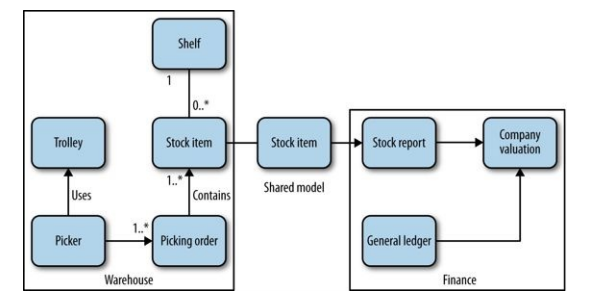
\includegraphics[width=10cm]{images/departements_relation.png}}	
		\captionof{figure}{Model pembagian dari departemen keuangan dan warehouse.}
	\end{minipage}
\end{adjustbox}

Untuk dapat menjalankan alur informasi, pegawai keuangan membutuhkan data stok. \textit{Stock item} menjadi \textit{shared model} antara dua departemen. Perlu diingat bahwa tidak semua data \textit{warehouse} harus diperlihatkan di keuangan, jadi terdapat representasi internal dan representasi external yang diperlihatkan. Desain diatas memperlihatkan konsep \textit{loose coupling} dan \textit{high cohesion} yang digambarkan menjadi sebuah modul. Desain seperti ini sangat mempermudah proses perpindahan dari monolitik dan menyakinkan bahwa desain microservice telah \textit{loosely coupled} dan \textit{stongly cohesive} \cite{9}.
\section{Integrasi Teknologi}
Mengintegrasikan dengan benar merupakan tahap yang paling penting, memungkinkan perubahan yang signifikan dengan tingkat kemandirian aplikasi yang tinggi. Dalam tahap integrasi ini ada beberapa point penting yang harus dianalisis sebelum memilih teknologi yang digunakan dan mengimplementasikannya.
\begin{enumerate}[leftmargin=*]
	\item \textit{\textbf{Menjaga teknologi API agar tetap agnostik.}} IT industri adalah berubah dengan sangat cepat, \textit{tools} baru, \textit{framework} dan bahasa baru, serta ide-ide implementasi yang selalu berkembang. Hal inilah yang menjadi pertimbangan agar memastikan bahwa API inisial harus dapat digunakan terus menerus ketika mengimplementasikan microservice.
	\item \textit{\textbf{Hindari perubahan major pada aplikasi.}} Perubahan arsitektur dapat mengakibatkan perubahan pada bagian-bagian aplikasi yang lainnya, pemilihan teknologi yang tepat bertujuan agar perubahan ini terjadi sekecil mungkin.
	\item \textit{\textbf{Buat service sederhana untuk dipakai.}} Arsitektur microservice yang baru harus cepat beradaptasi dengan penggunanya, maka dari itu modul service harus bersifat \textit{user-friendly}. 
\end{enumerate}
Seperti yang dikutip dari website Chris Richardson, microservice merupakan sekumpulan teknologi yang saling bekerjasama. Teknologi tersebut tidak dibatasi oleh sebuah wadah tertentu, namun saling terpisah yang menyebabkan luasnya pemilihan teknologi yang akan digunakan. Point berikutnya akan menjelaskan beberapa pilihan teknologi yang baik yang dapat diimplementasikan. Mulai dari lapisan paling dalam, yaitu managemen data, pembagian service, metode berkomunikasi antar service, sampai dengan API gateway yang akan digunakan oleh clien \cite{9}.
\subsection{Manajemen Data}
Bab ini akan membahas bagaimana penyimpanan data pada arsitektur monolitik dan apa kelemahannya. Kemudian dilanjutkan dengan penjelasan dan pembahasan metode penyimpanan data yang baik dan sesuai dengan arsitektur microservice.
\subsubsection{Model Penyimpanan Data Arsitektur Monolitik}
Pada arsitektur biasa, umumnya database disimpan dalam 1 tempat dan terdiri dari beberapa table. Ketika terjadi permintaan untuk membaca data, maka sistem akan mengambil data tersebut dari database, sama halnya apabila data diubah, maka sistem akan langsung mengubah database. \textit{Life cycle} seperti ini sangat simpel dan sangat cepat sehingga sampai saat ini dipakai oleh banyak sistem.\\
Contoh dalam gambar 2-1, \textit{customer} yang akan melakukan registrasi akan melakukan \textit{querry} ke database, juga aplikasi \textit{call center} yang menampilkan dan mengubah data akan langsung melakukan \textit{querry} ke database, begitu pula dengan informasi \textit{update warehouse} mengenai pesanan konsumen, akan melakukan \textit{query} pada database. Ini adalah contoh pattern yang sangat umum, namun banyak kelemahan dari pattern database ini \cite{9}

\begin{adjustbox}{width=1\textwidth}
	\centering
	\begin{minipage}{\linewidth}
		\framebox[\textwidth]{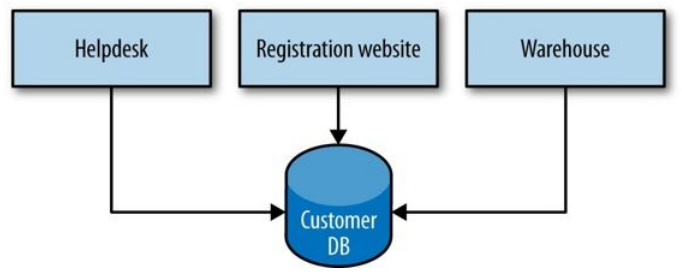
\includegraphics[width=10cm]{images/common_accessing_db.png}}	
		\captionof{figure}{Pemodelan cara akses database yang umum.}
	\end{minipage}
\end{adjustbox}\\

Pertama, model ini mengizinkan langsung pihak luar untuk mengubah data internal. Struktur data yang di simpan di DB dipakai oleh semua \textit{user}, apabila terjadi perubahan pada DB, maka semua \textit{user} akan terkena dampaknya. Database menjadi sangat besar, dan \textit{shared} API menjadi rapuh. Apabila akan terjadi perubahan, misalnya perubahan table customer di database, maka harus sangat berhati-hati agar \textit{schema} yang dipakai oleh service lain tidak rusak. Hal ini membutuhkan usaha testing regresi yang besar. Hal ini melanggar konsep \textit{loose coupling} \cite{9}. Kedua, semua \textit{client} menjadi terikat dengan sebuah teknologi spesifik. Mungkin saat ini database berjalan dengan baik dengan menggunakan \textit{relational} database, namun bagaimana bila seiring berjalannya waktu, performa untuk menyimpan data lebih baik menggunakan \textit{nonrelational} database? \textit{Client} menjadi terikat dengan model implementasi. Hal ini melanggar konsep \textit{cohesion}.
\subsubsection{Model Penyimpanan Data Arsitektur Micoservice}
Dalam perancangan arsitektur microservice, terdapat 2 pattern database ditinjau dari pembagian database tersebut. Pattern pertama adalah \textit{shared database} dan yang kedua adalah \textit{database per service}. Untuk contoh kedua pattern, penulis Chris Richardson memberikan contoh dengan menggunakan modul \textit{customer} dan modul \textit{order}. Hubungan kedua modul tersebut terjadi ketika ada transaksi baru, dimana modul \textit{order} harus memastikan bahwa jumlah pesanan yang baru tidak melebihi limit kredit yang dimiliki \textit{customer}. Relasi kedua modul itu dapat dilihat dari gambar dibawa \cite{6}\\

\begin{adjustbox}{width=1\textwidth}
	\centering
	\begin{minipage}{\linewidth}
		\framebox[\textwidth]{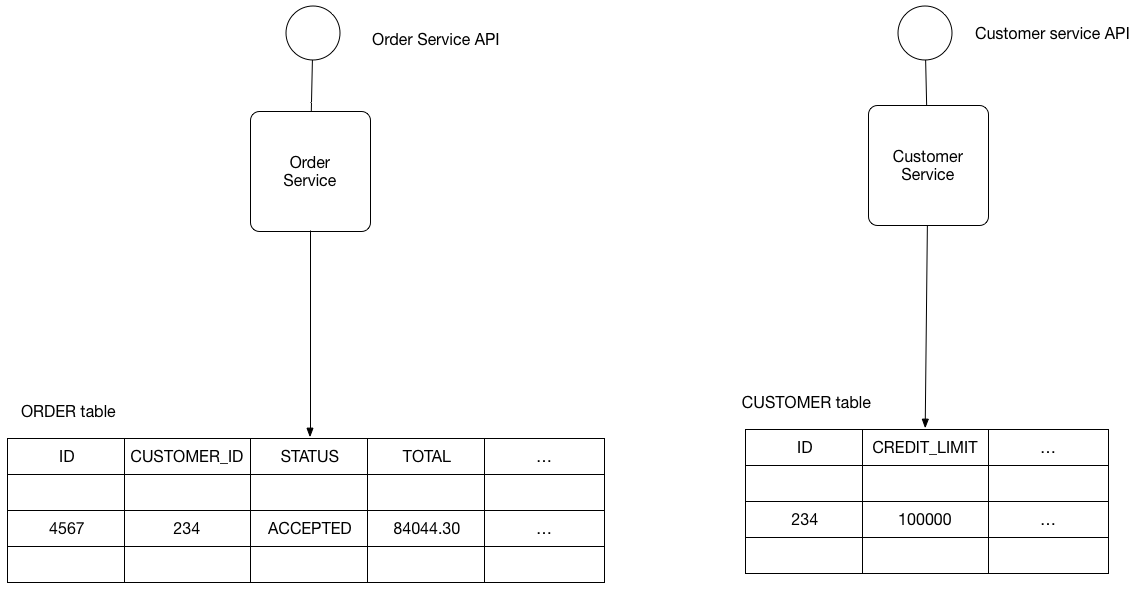
\includegraphics[width=13cm]{images/shared_database.png}}	
		\captionof{figure}{\textit{Shared database.}}
	\end{minipage}
\end{adjustbox}\\

\textbf{Shared database.} Model yang pertama adalah database yang di \textit{share} untuk diakses oleh beberapa service. Modul \textit{order} bisa langsung mengakses table \textit{customer} untuk mendapatkan limit kredit \textit{customer} tersebut. Model ini dapat menjadi pilihan ketika \textit{developer} ingin model yang familiar dan tegas untuk menjaga konsistensi data. Model \textit{shared database} memiliki beberapa kelemahan, antara lain :
\begin{enumerate}[leftmargin=*]
	\item \textit{Development time coupling.} Modul \textit{order} harus tahu apabila terjadi perubahan pada \textit{schema customer}, hal ini menjadikan kedua modul menjadi memiliki ketergantungan. Hal ini akan memperlambat proses \textit{development}.
	\item \textit{Runtime coupling.} Karena beberapa service dapat mengakses database yang sama, terdapat potensi mengganggu proses yang lain, misalnya ketika modul \textit{customer} sedang melakukan \textit{update} terhadap \textit{customer} dengan id 234 untuk merubah kredit limit, maka modul \textit{order} harus menunggu sampai \textit{update customer} selesai dilakukan karena \textit{customer} dengan id 234 akan di \textit{block} sementara waktu.
\end{enumerate}
\textbf{Database per service}. Pattern database yang kedua menjadikan sebuah table menjadi \textit{private} hanya untuk 1 buah service dan hanya dapat diakses via API, service lain tidak bisa mengakses database tersebut. Kelebihan dari model ini adalah menjadikan service lebih \textit{loose coupled}, tingkat ketergantungan antar service rendah. Tiap service pun dapat memiliki database yang cocok untuk dirinya sendiri. Namun model database ini memiliki beberapa kesulitan, antara lain :
\begin{enumerate}[leftmargin=*]
	\item Mengimplementasikan proses bisnis yang melibatkan banyak service menjad lebih sulit, dan lebih baik dihindari karena akan menemukan kesulitan di integritas data, terutama database modern (NoSQL). Solusi terbaik adalah dengan menggunakan konsep SAGA pattern (dibahas pada point berikutnya), yang menjalankan \textit{event} ketika ada perubahan data. Service lain yang men-\textit{subscribe event} tersebut akan merespon dan melakukan \textit{update} \cite{6}.
	\item Mengimplementasi \textit{query} yang menggabungkan data dari banyak database akan lebih sulit \cite{6}.
\end{enumerate}
\subsection{\textit{API Composition}}
Ketika mengaplikasikan arsitektur microservice menggunakan pattern \textit{database per service}, praktis implementasi dari \textit{straightforward query} yang menggabungkan data lebih dari satu tabel tidak dapat dilakukan lagi, karena tabel dalam database terpisah di berbagai lokasi service. Solusi untuk dapat mengatasi permasalahan ini adalah dengan menggunakan \textit{API Composition}. Ide dari konsep ini adalah menggabungkan data hasil service dan melakukan \textit{in-memory} join di level sistem. Namun kelemahan dari metode ini adalah menyebabkan data join yang besar dalam \textit{memory} system. Untuk menangani masalah tersebut, dapat dilakukan dengan meningkatkan performa \textit{hardware}, misal menambah \textit{core} dari \textit{processor} dan menambah \textit{memory} sistem \cite{6}.

\begin{adjustbox}{width=1\textwidth}
	\centering
	\begin{minipage}{\linewidth}
		\framebox[\textwidth]{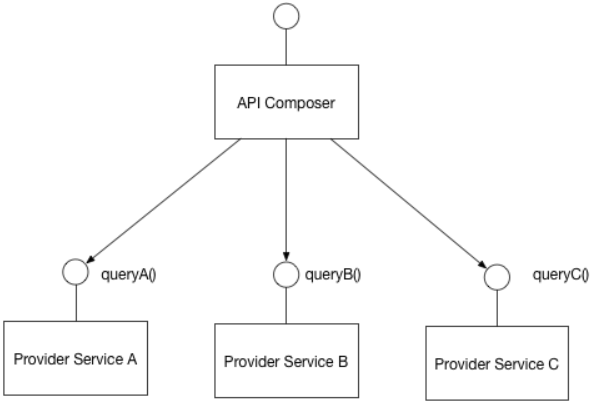
\includegraphics[width=10cm]{images/api_composition.png}}	
		\captionof{figure}{Meminta data dari service yang dibutuhkan dan melakukan \textit{in-memory join}}
	\end{minipage}
\end{adjustbox}
\subsection{Dekomposisi Modul}
Tujuan dari dekomposisi modul ini adalah menemukan service terkecil penyusun aplikasi. Dengan memisahkan modul menjadi sebuah service tunggal, menjadikan aplikasi lebih mandiri dan mudah untuk di koordinasikan dalam tim, yang dapat mempercepat proses \textit{development}. Tujuan yang lebih besar lagi adalah menghindari perubahan besar pada aplikasi ketika ada proses bisnis yang berubah. Dengan mendekomposisi modul, akan membantu untuk memastikan hanya ada sebuah service saja yang akan terkena dampaknya.\\
Tantangan yang didapat ketika hendak melakukan dekomposisi modul adalah :
\begin{enumerate}[leftmargin=*]
	\item Rancangan arsitektur service yang baru harus stabil.
	\item Sebuah service harus terdiri dari susunan \textit{functions} yang erat fungsinya.
	\item Service harus memastikan tidak melanggar \textit{Common Closure Principle}, yaitu apabila terjadi perubahan tidak akan melibatkan \textit{package} lain.
	\item Setiap service sebagai API yang terenkapsulasi dari pengguna. Segala perubahan tidak boleh memberikan dampak secara langsung pada pengguna.
	\item Sebuah service harus cukup kecil untuk ditangani oleh tim yang terdiri dari 6-10 orang.
	\item Service harus bisa di tes, dan setiap tim harus dapat melakukan proses \textit{develop} dan \textit{deploy} tanpa banyak interaksi dengan tim lain.
\end{enumerate}
Terdapat 2 metode dalam mendekomposisi modul aplikasi, yaitu berdasarkan subdomain dan berdasarkan proses bisnis yang dilakukan \cite{6}.\\
\textbf{Dekomposisi berdasarkan subdomain.} Apabila aplikasi yang dibentuk terpisah berdasarkan \textit{domain-driven design} (DDD) atau disebut juga subdomain, maka metode ini dapat lebih mudah digunakan. DDD memisahkan aplikasi berdasarkan kebutuhannya dan membentuk sebuah subdomain sendiri, setiap subdomain bertanggung jawab untuk menangani proses bisnis yang berbeda.Subdomain dapat diklasifikasikan sebagai berikut :
\begin{enumerate}[leftmargin=*]
	\item \textit{Core} – kunci pembeda dari proses bisnis dan menjadi bagian yang sangat penting dari sebuah aplikasi.
	\item \textit{Supporting} – berhubungan dengan proses bisnis namun bukan menjadi pembeda.
	\item \textit{Generic} – tidak berhubungan dengan proses bisnis dan biasanya hanya menjadi proses pendukung saja.
\end{enumerate}
Kelebihan dari metode ini antara lain:
\begin{enumerate}[leftmargin=*]
	\item Arsitektur service baru yang stabil, karena subdomain sendiri secara relatif sudah stabil.
	\item Service yang dibentuk akan cenderung memenuhi \textit{loosely coupled} dan \textit{cohesive}.
\end{enumerate}
Masalah yang dihadapi dari metode ini antara lain:
\begin{enumerate}[leftmargin=*]
	\item Sulit diterapkan untuk aplikasi yang tidak \textit{domain-driven} atau aplikasi yang memiliki keterikatan modul yang kuat.
\end{enumerate}
\textbf{Dekomposisi berdasarkan proses bisnis.} Pattern alternatif yang lain adalah mendefinisikan service berdasarkan kemampuan bisnis. Kemammpuan bisnis adalah proses yang dilakukan untuk menghasilkan sebuah nilai. Kemampuan bisnis biasanya berhubungan dengan objek bisnis. Misalnya \textit{order management} bertanggung jawab untuk \textit{orders}, \textit{customer management} bertanggung jawab untuk \textit{customer}.  Kemampuan bisnis biasanya tersusun menjadi hirarki multi level, misalnya untuk aplikasi perusahaan memiliki \textit{product/service development}, setelah itu ada \textit{product/service delivery}, lalu diikuti dengan \textit{aftersale service} \cite{6}
Kelebihan dari metode ini antara lain:
\begin{enumerate}[leftmargin=*]
	\item Arsitektur service baru yang stabil, karena kemampuan bisnis pun relatif sudah stabil.
	\item Service yang dibentuk akan memenuhi konsep \textit{loosely coupled} dan \textit{cohesive}.
\end{enumerate}
Masalah yang akan dihadapi dari metode ini antara lain:
\begin{enumerate}[leftmargin=*]
	\item Sulit untuk mengidenfitikasi kemampuan bisnis aplikasi. Identifikasi pembentukan service membutuhkan pemahaman dari proses bisnis, maka harus dilakukan analisa mendalam dari tujuan perusahaan, struktur, dan cakupan area. Analisa dapat dilakukan pertama-tama dari struktur organisasi, karena perbedaan grup dalam organisasi berkaitan dengan kemampuan bisnis dari grup tersebut.
\end{enumerate}
\subsection{Service Deployment}
Setelah mengindentifikasi dan membentuk service, tahap selanjutnya yang akan dilakukan adalah melakukan \textit{deployment} service untuk nantinya digunakan. Tiap service sendiri bisa ditulis menggunakan bahasa dan framework yang berbeda-beda, namun secara mandiri harus \textit{deployable} dan \textit{scalable}. Dalam beberapa kasus, akan terdapat set service yang harus terisolasi dari service lainnya. Kebutuhan lainnya adalah adanya keperluan untuk dapat memantau penggunaan \textit{resources} (CPU dan memori) yang digunakan oleh service dan memantau dengan mudah sifat dan kegunaan dari service tersebut. Semua kebutuhan ini juga harus sebanding dengan biaya yang dikeluarkan.\\
Terdapat beberapa metode \textit{deployment} yang dapat dilakukan, tiap metode cocok digunakan sesuai dengan kebutuhan dari \textit{deployment} itu sendiri. Point berikutnya akan menjelaskan metode-metode \textit{deployment} service.
\begin{enumerate}[leftmargin=*]
	\item \textbf{Multiple service instances per host.}\\
	Metode \textit{deployment} ini cocok digunakan apabila service yang terbentuk tidak banyak dan adanya kebutuhan untuk menghemat penggunaan sumber daya. Set service yang terbentuk disimpan dalam sebuah host (fisik atau \textit{virtual machine}). Terdapat 2 cara dalam melakukan \textit{deploy} set service dalam sebuah host. Pertama, \textit{deploy} set-set service tersebut sebagai JVM, misalnya dengan Tomcat atau Jetty untuk sebuah set service. Kedua adalah melakukan \textit{deploy} semua set service dalam sebuah JVM yang sama, mislanya sebagai web aplikasi \cite{6}.\\
	Metode deployment ini juga terdapat beberapa kelemahan, antara lain:
	\begin{enumerate}[leftmargin=*]
		\item Beresiko terjadi konflik terhadap kebutuhan sumber daya (memori dan CPU).
		\item Beresiko terjadi konflik versi dependency.
		\item Sulit untuk membatasi konsumsi sumber daya yang digunakan sebuah service (berhubungan dengan point pertama).
		\item Apabila banyak set service di deploy dalam sebuah mesin yang sama, maka akan sulit untuk memonitor konsumsi sumber daya dari tiap service, karena sulit untuk melakukan isolasi terhadap service.
	\end{enumerate}
	\item \textbf{Single service instance per host.}\\
	Pilihan yang kedua adalah setiap service memiliki hostnya sendiri. Dengan menerapkan pattern ini, setiap service akan terisolasi dari yang lainnya, serta tidak akan ada resiko konflik akan sumber daya dan dependency. Setiap service lebih mudah untuk dimonitor dan dikelola. Namun kekurangan dari patern ini apabila dibandingkan dengan multiple service per host adalah kurangnya efisiensi penggunaan sumber daya, karena bisa jadi akan ada banyak host yang digunakan \cite{9}
	
\begin{adjustbox}{width=1\textwidth}
	\centering
	\begin{minipage}{\linewidth}
		\framebox[\textwidth]{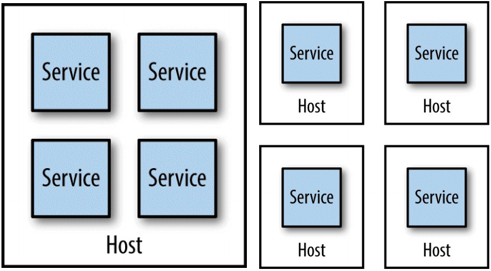
\includegraphics[width=8cm]{images/service_deployment.png}}	
		\captionof{figure}{\textit{Banyak service per host dan satu service per host.}}
	\end{minipage}
\end{adjustbox}\\
	\item \textbf{Service instance per container.}\\
	Apabila masing-masing service dibuat dengan bahasa atau framework yang berbeda, maka proses \textit{deployment} dari setiap service akan berbeda-beda pula. Dengan menggunakan \textit{container}, semua detail teknologi yang digunakan oleh setiap service akan dibuat terenkapsulasi dari service lain. \textit{Container} juga menspesifikasikan dengan jelas bagaimana proses \textit{deployment} yang harus dilakukan dalam sebuah mesin, sehingga ketika sebuah aplikasi hendak dijalankan dalam mesin yang berbeda, user tidak perlu tahu proses apa saja yang harus dilakukan [9].  Contoh dari \textit{container} adalah Docker, namun Docker tidak bisa melakukan \textit{deployment} dalam banyak mesin. Maka dari itu Google mengembangkan \textit{tools} yang bernama Kubernetes, Kubernetes memungkinkan agar Docker bisa dalam satu saat bersamaan dijalankan dalam banyak mesin sekaligus \cite{9}
	
\begin{adjustbox}{width=1\textwidth}
	\centering
	\begin{minipage}{\linewidth}
		\framebox[\textwidth]{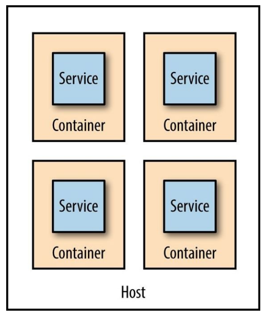
\includegraphics[width=5cm]{images/container_deployment.png}}	
		\captionof{figure}{\textit{Menggunakan container untuk \textit{deployment}.}}
	\end{minipage}
\end{adjustbox}\\
	\item \textbf{Serverless deployment.}\\
	Ide dari serverless deployment adalah mengurangi interaksi dari pengguna dengan server. Segala hal yang berhubungan dengan infrastruktur server disembunyikan dari pengguna. Pengguna hanya dikenakan biaya penyewaan server saja, namun tidak perlu lagi melakukan pengaturan apapun pada server. Untuk melakukan deployment, pengguna meembuat package dari kode (misalnya ZIP file), lalu melakukan upload kepada penyedia jasa server dan melakukan pengaturan performa. Ada beberapa penyedia jasa lingkungan serverless, misalnya AWS Lambda, Google Cloud Function, Microsoft Azure \cite{6}.\\
	Kelebihan dari penggunaan serverless ini antara lain:
	\begin{enumerate}[leftmargin=*]
		\item Tidak perlu membuang-buang waktu untuk mengurus menejemen infrastruktur low-level. Pengguna bisa lebih fokus untuk mengembangkan aplikasinya saja.
		\item Arsitektur dari serverless sangat elastis. Server secara otomatis menghitung beban dari service yang digunakan agar tidak ada resource yang terbuang.
	\end{enumerate}
	Kekurangan dari serverless antara lain:
	\begin{enumerate}[leftmargin=*]
		\item Adanya batasan lingkungan, misalnya server hanya bisa support untuk beberapa bahasa saja.
	\end{enumerate}
\end{enumerate}
\subsection{Metode Berkomunikasi Antar Service}
Dengan memiliki modul service yang berbeda-beda, timbul sebuah masalah yang berkaitan dengan pertukaran informasi yang berasal dari banyak service. \textit{Remote Procedure Invocation} (RPI) adalah protocol yang menyediakan teknik komunikasi antara service yang berbeda lokasi. Teknologi RPI ini ada yang menggunakan kode biner sebagai format pertukaran data, ada pula yang menggunakan format pesan XML seperti SOAP. Implementasi RPI ini berguna untuk mendapatkan data dengan sangat cepat yang dikirimkan melalui jaringan, hal yang menjadi keuntungan utama dari RPI adalah kemudahan penggunaannya. Contoh RPI lain yang menjadi fokus disini adalah Representational State Transfer (REST), point berikutnya akan menjelaskan mengapa REST menjadi pilihan terbaik untuk menangani proses komunikasi di microservice \cite{9}.

\textbf{Representational State Transfer (REST).} REST adalah standar arsitektur web yang menggunakan protokol HTTP. HTTP sendiri mempunyai kemampuan yang sangat cocok untuk REST, salah satunya HTTP faham apa yang harus dilakukan apabila menerima perintah GET, POST, PUT dari REST. Kelebihan penting yang dimiliki REST adalah pengguna bisa menghindari kontak langsung dari pengguna dengan server secara langsung. Konsep ini kemudian disebut sebagai \textit{hypermedia as the engine of application state} (HATEOAS). \textit{Hypermedia} adalah konsep dimana sebuah konten mempunyai link yang berhubungan dengan konten lainnya yang bisa berupa berbagai format (text, gambar, suara) \cite{9}. Ide dari HATEOAS adalah \textit{client} berhubungan dengan server hanya dengan menggunakan \textit{link} yang telah disediakan. 
Misalnya seperti gambar 2.6 dibawah. Ketika pengguna ingin mengubah data \textit{account}, maka pengguna akan mengirimkan \textit{request} pada \textit{account service}, \textit{account service} dengan logic yang dimilikinya akan menentukan apakah request tersebut dapat diterima. \textit{Account service} disini menjaga semua interaksi yang berhubungan dengan data \textit{account} itu sendiri. \textit{Client} tidak perlu tahu dan tidak perlu beradaptasi apabila terjadi perubahan pada server. \textit{Client} akan merasakan perubahan hanya apabila terjadi perubahan sifat atau ketika hilangnya kontrol yang merepresentasikan \textit{account}. Format data yang dikirimkan REST di HTTP dapat beragam, namun yang paling populer adalah format JSON, karena JSON mudah dimengerti dan mudah dikonsumsi langsung. REST pada HTTP sangat baik untuk diimplementasikan pada interaksi \textit{sevice-to-service} \cite{9}\\

\begin{adjustbox}{width=1\textwidth}
	\centering
	\begin{minipage}{\linewidth}
		\framebox[\textwidth]{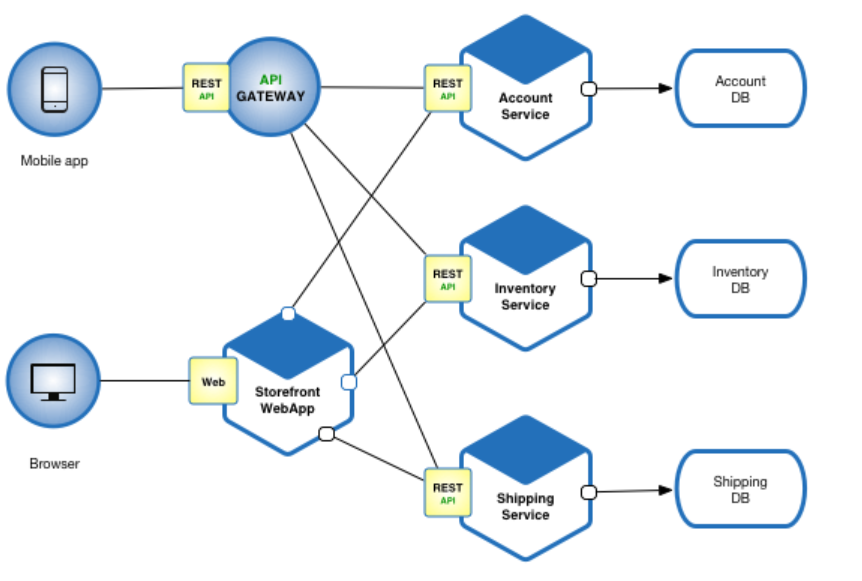
\includegraphics[width=12cm]{images/rest_example.png}}	
		\captionof{figure}{\textit{Contoh pemanfaatan REST sebagai media user-server}}
	\end{minipage}
\end{adjustbox}\\
\section{Strategi Pengujian}
Strategi pengujian berguna untuk memberikan gambaran dari test yang akan dilakukan terhadap \textit{software}. Testing ini berguna untuk memberi tahu kepada proyek menejer, tester, dan tim pengembang apabila ditemukannya masalah dalam \textit{software}. Strategi pengujian ini termasuk tujuan dari test, metode yang digunakan, sumber daya yang digunakan, juga lingkungan ketika menjalankan proyek. Test strategi mendeskripsikan seberapa tinggi resiko kesalahan (kegagalan) yang dapat terjadi \cite{12}. 
\subsection{Pengujian Arsitektur Microservice}
Uji kelayakan arsitektur microservice menurut Martin Fowler adalah dengan melakukan 5 test yang mirip dengan software testing pada umumnya, test tersebut antara lain adalah:
\begin{enumerate}[leftmargin=*]
	\item \textit{Unit Testing}. Bagian terkecil dalam software yang ditest untuk menentukan apakah unit tersebut bekerja sesuai harapan. Umumnya, unit yang dimaksud adalah kelas penyusun atau grup kecil yang menghubungkan kelas-kelas tersebut dan method yang terdapat dalam kelas.
	\item \textit{Integration Testing}. Goal dari test ini adalah membuktikan bahwa tidak terdapat masalah dari komunikasi dan interaksi dari setiap unit.
	\item \textit{Component Testing.} Komponen membatasi lingkup sebuah software. Dalam 1 buah komponen, dapat terdiri dari beberapa integrasi yang terjadi antara unit kelas.
	\item \textit{Contract testing.} Test yang memverifikasi bahwa pihak luar yang mengakses sebuah service akan mendapatkan hasil yang sesuai dengan harapan.
	\item \textit{End-to-end Testing.} Memverifikasi bahwa sistem memenuhi telah berhasil memenuhi kebutuhan dan sesuai dengan rancangan goal. Test dilakukan dari awal sampai dengan output yang dihasilkan. 
\end{enumerate}
\begin{adjustbox}{width=1\textwidth}
	\centering
	\begin{minipage}{\linewidth}
		\framebox[\textwidth]{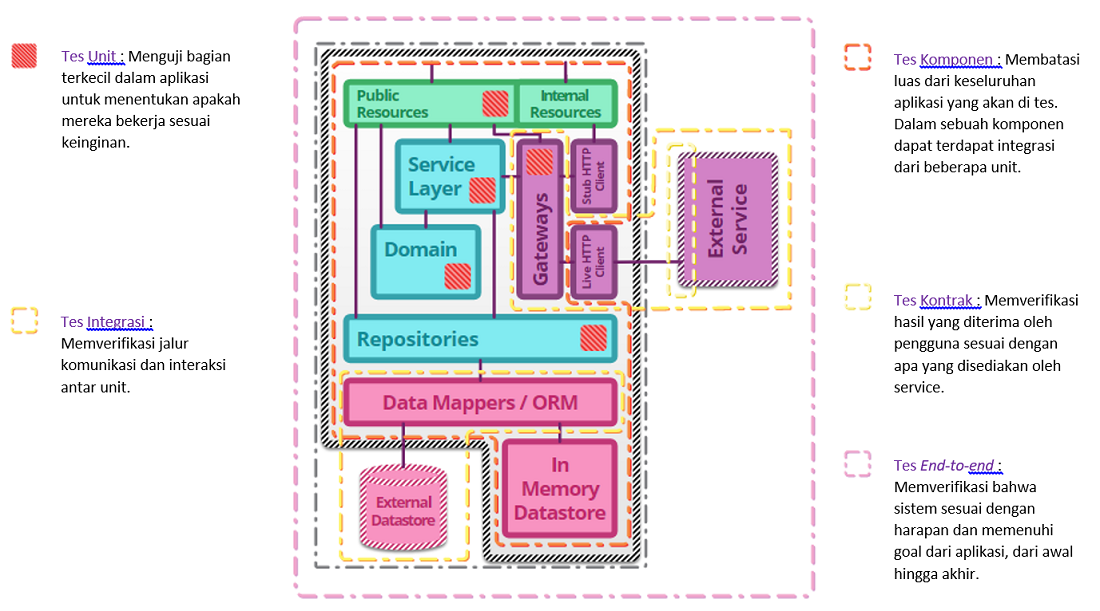
\includegraphics[width=13cm]{images/software_test.png}}	
		\captionof{figure}{\textit{Testing pada software microservice}}
	\end{minipage}
\end{adjustbox}\\

Tujuan utama dari testing yang pertama adalah memastikan bahwa fungsi bisnis dari arsitektur yang baru sudah memenuhi \textit{requirement} yang sama dengan arsitektur monolitik sebelumnya.
\subsection{Perbandingan Arsitektur}
Perbandingan arsitektur bertujuan untuk membuktikan arsitektur microservice yang dirancang akan memberikan hasil yang lebih baik dari arsitektur sebelumnya. Menurut Susan J. Fowler pada bukunya yang berjudul Microservices in Production "Standard Principles and Requirements", perbandingan akan dilakukan dengan mengacu pada 5 faktor, yaitu performa, stabilitas, availabilitas, reliabilitas, dan skalabilitas \cite{10} .
\begin{enumerate}[leftmargin=*]
	\item \textit{Performa}. Kemampuan sistem untuk menangani masalah yang diberikan dan seberapa efisien sistem menggunakan sumber daya yang tersedia (seperti \textit{hardware} dan komponen infrastruktur lainnya). 
	\item \textit{Stabilitas}. Sistem harus dipastikan selalu memberikan kondisi yang aman untuk tahap \textit{development, deployment}, sampai tahap pengenalan. 
	\item \textit{Availabilitas}. Perbandingan waktu \textit{downtime} dan \textit{uptime} dari sistem. \textit{Downtime} adalah total waktu aplikasi tidak bekerja sedangkan \textit{uptime} adalah total waktu sistem bekerja dengan baik. Tingkat availabilitas dihitung dari \textit{uptime} dibagi dengan \textit{downtime} + \textit{uptime}. Tingkat availabilitas dapat digunakan untuk melihat seberapa baik sistem bekerja.
	\item \textit{Reliabilitas}. Sebuah sistem yang \textit{reliable} harus dapat memberikan data yang dapat dipercaya oleh \textit{clients} dan ekosistem tempat sistem itu berada. \textit{Request} dan \textit{response} harus sampai tepat pada tujuan dan \textit{error} harus dapat diatasi secara benar dan aman.
	\item \textit{Skalabilitas}. Kemampuan sistem untuk menangani permintaan yang besar dalam satu waktu bersamaan. Untuk dapat memastikan bahwa sistem \textit{scalable}, perlu diketahui seberapa besar ukuran sistem secara kuantitatif (misal seberapa banyak \textit{request} per detik yang dapat ditangani sistem).
\end{enumerate}
\section{Tinjauan Studi}
\begin{small}
	\begin{longtable}{@{\extracolsep{\fill}}|p{0.5cm}|p{2cm}|p{2cm}|p{1cm}|p{3.70cm}|}
		\caption{Tabel Tinjauan Studi}\\
		\hline
		\textbf{No } & \textbf{Peneliti} & \textbf{Judul} & \textbf{Tahun
		} & \textbf{Konsep}\\
		\hline
		\endhead
		1 & Sam Newman & \textit{Building Microservice} & 2015 & Menjelaskan pendekatan yang paling tepat untuk membangun service yang saling berkolaboratif dan memberi panduan untuk mengintegrasikan teknologi agar menjadi padu dengan service yang dibangun.\\
		\hline
		2 &  Susan J. Fowler & \textit{Microservices in Production} & 2017 & Menjelaskan standar dan goal yang harus dicapai dari perancangan microservice. Standar yang harus dipenuhi tersebut terdiri dari performa, stabilitas, availabilitas, reliabilitas, dan skalabilitas. \\
		\hline
		3 & K. Siva Prasad Reddy & \textit{Beginning
			Spring Boot 2} & 2017 & 
		Memberikan panduan untuk membangun \textit{web service} menggunakan REST API dan bekerja dengan \textit{NoSQL database} menggunakan framework java yang bernama Spring. \\
		\hline
		4 & Chris Richardson  & \textit{Microservices Patterns} & 2017 & 
		Memberikan panduan untuk melakukan migrasi sistem dari arsitektur monolitik menjadi arsitektur microservice. Menjelaskan teknologi yang dapat diintegrasikan dengan microservice dan cara implemetasinya. \\
		\hline
	\end{longtable}		
\end{small}

Pada penelitian satu, Sam Newman memulai dengan memberikan pengenalan dari microservice lalu dilanjutkan dengan keuntungan dan kerugian dari arsitektur tersebut. Kemudian Sam Newman melanjutkan dengan memberikan cara untuk memodelkan service menggunakan \textit{domain-driven} desain untuk membantu analisa berpikir. Tahap selanjutnya menjelaskan integrasi teknologi yang dapat membantu perancangan desain. Pada bagian akhir Sam Newman memberikan contoh \textit{splitting}  monolitik menjadi microservice dan bagaimana \textit{deployment} dilakukan \cite{9}.

Pada penelitian dua, Susan J. Fowler menjelaskan bahwa terdapat 5 standar yang menjadi parameter microservice dapat dinyatakan berhasil pada tahap \textit{production}. Ke 5 standar tersebut adalah availabilitas yang dapat ditunjukan dengan seberapa lama waktu \textit{downtime} yang terjadi pada sistem. Stabilitas yang ditunjukan dengan kestabilan dari sisi \textit{development, deployment,} dan tahap pengenalan. Reliabilitas yang dapat ditunjukan dengan proses \textit{deployment} yang terjamin, \textit{planning} dan perlindungan ketika terjadi kegagalan pada sistem dan tingkat keamanan dari segi pertukaran data. Skalabilitas yang menunjukan bahwa pertumbuhan sistem dapat didefinisikan secara kuantitatif, identifikasi sumber masalah \textit{bottlenecks}, dapat direncanakan kapasitas yang dibutuhkan sistem, dan dapat \textit{data storage} yang dapat diprediksi. Performa yang dapat dilihat dari kemampuan sistem menangani masalah yang diberikan dan seberapa efisien sistem menggunakan sumber daya yang tersedia \cite{10}.

Pada penelitian tiga, \textit{Beginning Spring Boot 2} memberikan panduan dalam menggunakan salah satu \textit{framework} populer dari java yaitu Spring \textit{framework}. Pada awal panduan, penulis memberi tahu pembaca untuk menyiapkan \textit{JDK 1.8}, \textit{IDE Netbeans} atau \textit{Eclipse}, \textit{build tools} seperti \textit{maven}, dan server basis data seperti \textit{MySQL} atau \textit{PostgreSQL}. K. Siva Prasad Reddy kemudian memulai penjelasan dari apa itu \textit{Spring Boot} dan bagaimana \textit{framework} ini dapat membantu produktivitas \textit{developer}, kemudian bagaimana \textit{auto configuration} dari Spring Boot bekerja dibelakang layar, dan bagaimana membuat \textit{Spring Boot starters}. Kemudian K. Siva Prasad Reddy melanjutkan pembahasan sampai bagaimana membuat \textit{Reactive Web Application} dan membuat REST API menggunakan \textit{Spring Boot} \cite{11}.

Pada \textit{chapter} pertama di penelitian empat, Chris Richardson mendeskripsikan arsitektur microservice serta kelebihan dan kekurangannya, serta bagaimana microservice dapat menyelesaikan masalah dari monolitik. \textit{Chapter} kedua menjelaskan bagaimana untuk merubah \textit{aplikasi} menjadi \textit{set of services} dengan menggunakan 2 strategi dekomposisi. \textit{Chapter} tiga menjelaskan REST API sebagai media komunikasi \textit{web service} dan bagaimana REST API bekerja. Pada \textit{chapter} terakhir Chris Richardson membahas cara \textit{deployment} microservice \cite{13}.

\section{Objek Penelitian}
Pada bagian ini akan dibahas objek-objek yang terkait dengan analisis penelitian.
\subsection{Perangkat Lunak}
Rekayasa perangkat lunak adalah sebuah profesi yang dilakukan oleh seorang perekayasa perangkat lunak yang berkaitan dengan pembuatan dan pemeliharaan aplikasi perangkat lunak dengan menerapkan teknologi dan praktik dari ilmu komputer, manajemen proyek, dan bidang-bidang lainnya. Perangkat lunak adalah instruksi langsung komputer untuk melakukan pekerjaan dan dapat ditemukan di setiap aspek kehidupan modern dari aplikasi yang kritis untuk hidup \textit{(life-critical)}, seperti perangkat pemantauan medis dan pembangkit tenaga listrik sampai perangkat hiburan, seperti video game. Banyak produk perangkat lunak berisi jutaan baris kode yang diharapkan dapat melakukan pekerjaan dengan baik dalam menghadapi perubahan kondisi. Semua perangkat lunak juga membutuhkan keandalan yang tinggi dan harus dihasilkan secara ekonomis. Teknik rekayasa perangkat lunak akan meningkatkan fungsionalitas dan efisiensi aplikasi dan juga kemudahan dan efisiensi dari pengembang perangkat lunak. Pelopor rekayasa perangkat lunak adalah Barry Boehm, Fred Brooks, CAR Hoare, dan David Parnas. \cite{14}

\subsection{Microservice}
Microservice adalah pendekatan untuk mendistribusikan sistem yang membantu mengoptimalkan penggunaan service dengan siklus hidup mereka sendiri namun secara bersamaan saling berkolaborasi. Microservice terutama dimodelkan pada domain bisnis untuk memecahkan masalah dari arsitektural tradisional. Microservice mengintegrasikan teknologi dan teknik yang muncul selama dekade terakhir yang diharapkan dapat membantu menghindari kebuntuan dari sebuah sistem \cite{9}.
\newpage